\documentclass[a4paper,11pt]{article}
\usepackage[utf8]{inputenc}
\usepackage[paper=a4paper, hmargin=1.5cm, bottom=1.5cm, top=3.5cm]{geometry}
\usepackage[T1]{fontenc}
\usepackage[spanish]{babel}
\usepackage[colorlinks=true, linkcolor=blue]{hyperref} %Links para el indice.
\usepackage{amsfonts}
\usepackage{verbatim}
\usepackage{listings}
\usepackage{caption}
\usepackage{subcaption}

\usepackage[section]{placeins}
\usepackage{float}
%\usepackage{adjustbox}
\usepackage{amsmath}
\usepackage{blindtext}
\usepackage{sidecap}
\usepackage{color}
\usepackage{graphicx}
\usepackage{algpseudocode}
\usepackage{wrapfig}

\usepackage{algorithm}
\usepackage{algpseudocode}
% \newcommand{\real}{\hbox{\bf R}}

\newcommand{\funcName}[1]{\textbf{\texttt{#1}}}


\title{Trabajo Práctico de Sistemas Operativos}

\begin{document}

\maketitle

\begin{center}
	Universidad de Buenos Aires - Departamento de Computaci\'on - FCEN
\end{center}

\vspace{2cm}
Integrantes:

\begin{itemize}
	\item Castro, Dami\'an L.U.: 326/11  \verb+ltdicai@gmail.com+
	\item Toffoletti, Luis L.U.: 827/11 \verb+luis.toffoletti@gmail.com+
	\item Zanollo, Florencia L.U.: 934/11 \verb+florenciazanollo@gmail.com+
\end{itemize}

\newpage

\tableofcontents

\newpage

\section{Introducción}

Una computadora moderna consiste de uno o m\'as procesadores, memoria, discos, impresoras y uno o varios dispositivos de entrada/salida. Adem\'as una computadora ejecuta programas que suelen intentar acceder a estos recursos y generalmente asumiendo que son los \'unicos que desean utilizarlos. Sin embargo esto casi nunca es cierto y suelen haber conflictos cuando dos procesos (programas en ejecuci\'on) acceden al mismo recurso. Para solucionar estas problem\'aticas se recurre a los sistemas operativos, que son aquellos que se encargan de coordinar el acceso a los recursos por parte de los procesos. Un sistema operativo es un proceso superior a todos los dem\'as y decide, siguiendo alguna normativa, en que momentos los procesos comunes se ejecutan. Se conoce a esta normativa como pol\'itica de \emph{scheduling}, y no hay una \'unica manera de definirla. Dependiendo de la situaci\'on puede que se prefiera pol\'iticas que permitan a los procesos mantener ocupado un recurso durante per\'iodos largos de tiempo mientras que otras pol\'iticas se valen en desalojar a las tareas y otorgarle los recursos a otra tarea. Se espera que un \emph{scheduler} trate de cumplir los siguientes objetivos:

\begin{itemize}
	\item Ecuanimidad (\emph{fairness}): que cada proceso reciba una dosis “justa” de CPU (para alguna definici\'on de justicia).
	\item Eficiencia: tratar de que la CPU est\'e ocupada todo el tiempo.
	\item Carga del sistema: minimizar la cantidad de procesos listos que est\'an esperando CPU.
	\item Tiempo de respuesta: minimizar el tiempo de respuesta percibido por los usuarios interactivos.
	\item Latencia: minimizar el tiempo requerido para que un proceso empiece a dar resultados.
	\item Tiempo de ejecuci\'on: minimizar el tiempo total que le toma a un proceso ejecutar completamente.
	\item Rendimiento (throughput): maximizar el n\'umero de procesos terminados por unidad de tiempo.
	\item Liberaci\'on de recursos: hacer que terminen cuanto antes los procesos que tiene reservados m\'as recursos.
\end{itemize}

Como se puede intuir, es imposible cumplir todos los objetivos a la vez, por lo tanto las pol\'iticas de \emph{scheduling} tienen sus ventajas y sus desventajas. Es el enfoque de este informe exhibir dichas pol\'iticas, su implementaci\'on en lenguaje \emph{C++} y mostraremos sus pros y sus contras con ejemplos.

\subsection{Simulador}

Para analizar las diferentes pol\'iticas de \emph{scheduling} utilizamos un modelo de computadora simplificado que consiste en los siguientes componentes:

\begin{itemize}
	\item Un lote de programas a ejecutar.
	\item Uno o varios n\'ucleos (\emph{cores}) de procesamiento, que se encargar\'an de hacer los c\'omputos de los procesos.
	\item Un \'unico dispositivo de entrada y salida que todos los procesos pueden utilizar si lo desean.
\end{itemize}

\subsubsection{Acciones del simulador}

El simulador provee a los procesos con tres acciones posibles:

\begin{itemize}
	\item $uso\_CPU$(\emph{n}) que indica que el proceso utilizar\'a el CPU durante \emph{n} ciclos de reloj.
	\item $uso\_IO$(\emph{n}) que indica que el proceso utilizar\'a un recurso de entrada/salida durante $n$ ciclos de reloj. Durante este tiempo el proceso no utiliza al procesador, as\'i que el \emph{scheduler} es libre de utilizar ese tiempo en otra tarea.
	\item $return$ que indica que el proceso ya termin\'o su ejecuci\'on. El \emph{scheduler} debe realizar las acciones necesarias para desalojar al proceso.
\end{itemize}

\subsubsection{Definici\'on de \emph{schedulers}}

Un \emph{scheduler} v\'alido ofrece las siguientes funcionalidades:
\begin{itemize}
	\item \funcName{load(pid)}: Carga un proceso con n\'umero de identificaci\'on \funcName{pid}. 
	\item \funcName{unblock(pid)}: Se realiza cuando un proceso con n\'umero de identificaci\'on \funcName{pid} deja de utilizar un recurso de entrada/salida y desea volver a usar el procesador.
	\item \funcName{tick(cpu,motivo)}: Se ejecuta por cada $tick$ del reloj del procesador \funcName{cpu} y el \funcName{motivo} indica que sucedi\'o con el \'ultimo proceso que estaba en ejecuci\'on.
\end{itemize}


\section{Pol\'iticas de \emph{scheduling}}

\subsection{Ej 1: TaskConsola}

\begin{algorithm}
 \caption{TaskConsola}
 \begin{algorithmic}[1]
 \Procedure{TaskConsola}{$n, bmin, bmax$}
   \State $srand(time(NULL))$ \Comment{seteo semilla de random}
   \For{$i\gets 0, n$}\Comment{n veces}
     \State{$random\_ number\gets modulo(rand(),\ bmax - bmin + 1) + bmin$}\Comment{[1]}
     \State{$Uso\_ IO(random\_ number)$}    
   \EndFor
 \EndProcedure
 \end{algorithmic}
\end{algorithm}

[1]: rand() retorna un número arbitrariamente grande.
Tomando su módulo en (bmax - bmin + 1) nos aseguramos que esté entre 0 y (bmax - bmin).\newline
Luego sumamos bmin, resultando un número entre bmin y bmax.

\subsection{Ej 2: Ejecutar TaskConsola con FCFS}

FCFS (First-Come First-Served) un scheduler simple en el cual los procesos son asignados al CPU en el orden en que estos lo requieren.\newline

\begin{wrapfigure}{l}{0.3\textwidth}
  \vspace{-30pt}
  \begin{center}
    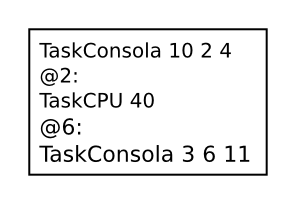
\includegraphics[width=0.25\textwidth]{./ej1y2/ej2_loteTareas.png}
  \end{center}
   \vspace{-30pt}
\end{wrapfigure}

Básicamente hay una sola cola (FIFO) de procesos 'Ready'. 
Cuando un proceso requiere CPU y éste está libre, se lo deja correr tanto tiempo como quiera y sin interrupciones.\newline

A continuación se muestran los gráficos para 1, 2 y 3 núcleos, usando SchedFCFS para el lote de tareas del cuadro.\newline

\vspace{10pt}
\textbf{1 Núcleo:}
\vspace{-20pt}
\begin{center}
 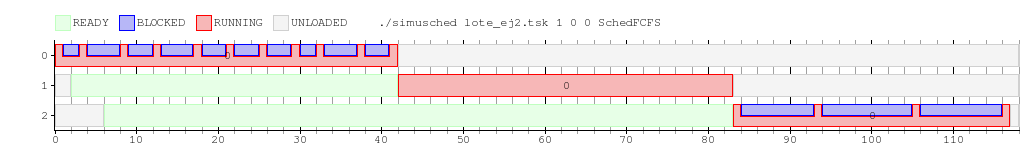
\includegraphics[scale=0.5]{./ej1y2/ej2_1core.png}
\end{center}

\vspace{10pt}

\textbf{2 Núcleos:}
\vspace{-20pt}
\begin{center}
 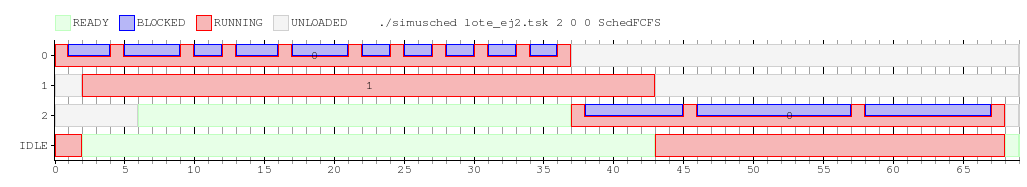
\includegraphics[scale=0.5]{./ej1y2/ej2_2core.png}
\end{center}

\vspace{10pt}

\textbf{3 Núcleos:}
\vspace{-20pt}
\begin{center}
 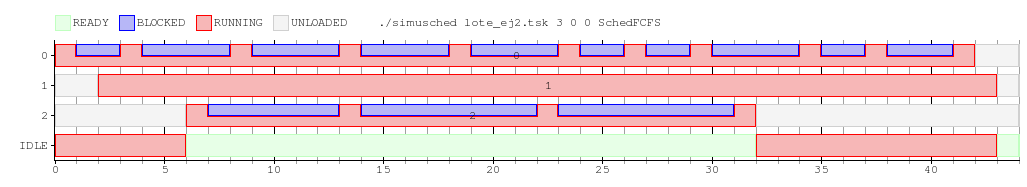
\includegraphics[scale=0.5]{./ej1y2/ej2_3core.png}
\end{center}


Obs: Los parámetros de costo de cambio de contexto y migración fueron seteados en 0 ya que en este scheduler en particular
no son tomados en cuenta. Porque núnca se desalojan las tareas ni se cambian de núcleo.

En los gráficos se hace evidente que a más cántidad de núcleos, mejor rendimiento, con FCFS.
Esto se debe a que FCFS no soporta múltitarea por sí sólo (ya que núnca desaloja a las tareas), sino que necesita varios núcleos para lograrlo.\newline

Las desventajas de FCFS son varias:

\begin{itemize}
\item Como ya dijimos, no soporta múltitarea.
\item Puede generar mucho 'waiting time'.\newline
	Si está ejecutando tareas muy largas las nuevas no entran hasta que éstas terminen.
\item No tiene buen rendimiento, a menos que se sepa la duración de las tareas de antemano.
\item Carece de 'fairness' i.e. no distribuye el/los procesador/es de forma justa entre las tareas.
\end{itemize}

\subsection{Ej 3: Round-Robin Implementación}
-Explicar la idea y la funcionalidad de c/u de las
estructuras de datos usadas
-Hacer pseudocódigo

\subsection{Ej 4: Round-Robin Simulaciones}

!Explicar por qué: 
-elegimos 1 costo cambio de contexto y 2 costo cambio de nucleo (hay una lista para todos los nucleos)
-es efectivamente un RR
-no siempre es mejor tener más núcleos en un RR con lista global
Esto depende de cuándo entren las tareas, que procesadores
estaban libres y el quantum de c/u

En estas im todos los cpu tienen quantum = 4
-Hacer otros experimentos con dif quantums y ver cuál queda mejor

\begin{center}
 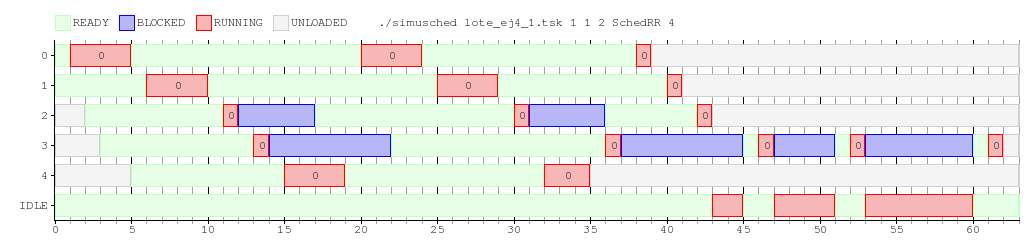
\includegraphics[scale=0.5]{./ej4/ej4_1cpu.png}
 % ej4_1cpu.png: 1027x247 pixel, 72dpi, 36.23x8.71 cm, bb=0 0 1027 247
\end{center}

\begin{center}
 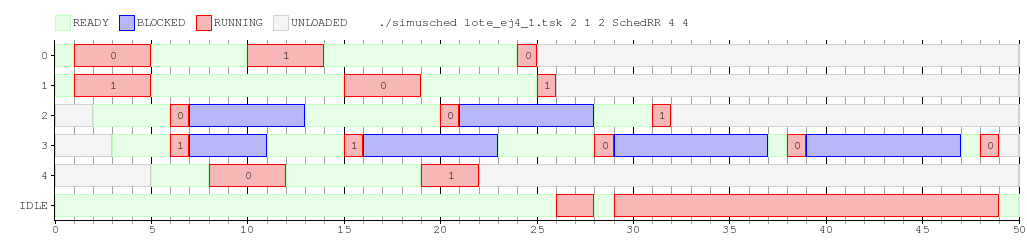
\includegraphics[scale=0.5]{./ej4/ej4_2cpu.png}
 % ej4_2cpu.png: 1027x247 pixel, 72dpi, 36.23x8.71 cm, bb=0 0 1027 247
\end{center}

\begin{center}
 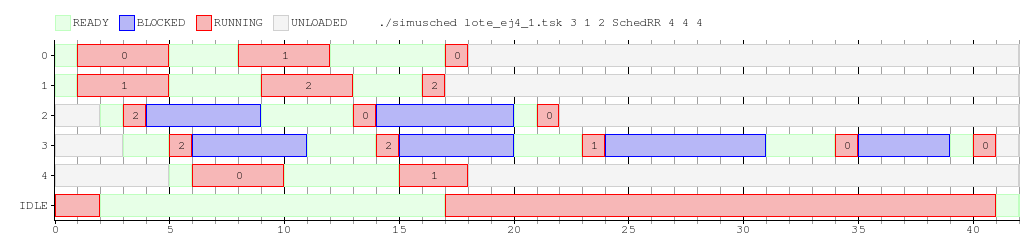
\includegraphics[scale=0.5]{./ej4/ej4_3cpu.png}
 % ej4_3cpu.png: 1027x247 pixel, 72dpi, 36.23x8.71 cm, bb=0 0 1027 247
\end{center}



\section{Discusi\'on}

\section{Conclusiones}


\end{document}
